%----------------------------------------------------------------
%
%  File    :  survey-CSS.tex
%
%  Author  :  Rok Kogovšek, TU Graz, Austria
% 
%  Created :  01 Dec 2016
% 
%  Changed :  X Dec 2016
% 
%----------------------------------------------------------------


\chapter{Cascading Style Sheets (CSS)}

\label{chap:CSS}

Knowing the usefulness of animation in web UI and the correct way of animation planing are just the fundemantals for our conceptual plans. Those still need to be implemented to get the end product and here we usually hit a wall build from the various tools, that say they can all solve our problems. Even well established people in the field have stories as such to tell. Val Head actually started with animation due to an interesting Flash workshop. Flash was at that time the de facto king in its era, however as we know, that era is already dead. Nowdays we can acomplish
all we could with Flash and more with just the core parts of the web, namely HTML, CSS and JS
\citep{head2016designing}.

\section{Do Everything You Can With CSS}

\label{sec:everythingCSS}

With Responsive web design (RWD) in our websites and animation being part of the design, see section \ref{sec:anime_dev}, it should be natural to use the guidelines of RWD also in animation planning. \citet{IAWEB} teaches us that one of the RWD guidelines is also Progressive enhancement, which is best described with words of the conceptual authors \citet{champeon2003inclusive}: {\em"Leave no one behind. . . .  accessibility is for everyone, not just the disabled"}. With CSS nowdays being a core part of the web and at the same time being the lowest web component that enables animation with RWD guidelines\footnote{Of course one can just use an animated image, e.q. a GIF with an image sequence, and just append it with HTML into the design. However, this image will become a static component of the design and will not follow RWD guidelines.}, one should always implement with CSS and HTML alone as much of the desired animation as possible. One has only to make sure the browser support for the animated attribute.

Other supporting arguments for use of CSS as the starting point for web UI animation beside responsiveness can be summarized with the the so called "Simple CSS Truths", a list of truths by \citet{palermoCSS} enhanced with the teachings of \citet{IAWEB}:

\begin{description}
\item [CSS allows for separation of concerns] -
 With CSS the form is separated from the page's HTML structure and content. Makes it easier to read, maintain and crawl the code.

\item [CSS has a captive audience] -
 Support for CSS development is huge. At the same time more and more libraries, tools and frameworks focus on improving and simplifing CSS development. 

\item [CSS is fast] - 
 External CSS speeds up HTML downlaod and loading compared to HTMLs with duplicated inline styles. Compared to JavaScript it also processes transitions and animations faster.

\item [CSS is fault-tolarent] - 
 Browser-unknown enhancements are simply ignored by the browser, while the remainder is still used and displayed.

\item [CSS is everywhere] - 
 Modern browsers embrace CSS and feature support by each can be easily found online.
\end{description}

% section everythingCSS (end)

\section{CSS Animation Declaration} % (fold)
\label{sec:declarationCSS}

As stated in section \ref{sec:anime_motion}, animation is about changing an element's attribute(s) over time. In CSS we can redefine it as a switch between CSS styles for a HTML element that happens gradually over time. It is stated that CSS animation should be done with {\em{}Animation} property(ies) and {\em{}Keyframe} rule(s). This may be the most efficient CSS way to accomplish animation, but CSS animation can also be achieved with {\em{}Transition} property(ies) and {\em{}selector} pattern(s)\citep{w3schoolAnime,w3schoolTrans}.


\subsection{Animation Property and Keframe Rule} % (fold)
\label{sub:CSS_animation_keyframe}

The prefered declaration for animation in CSS is done by setting animation properties to the element, that will change through time. This properties just define to which animation steps or keyframes the element is linked to and how the in-between-keyframe states are interpolated through time. \citet{w3schoolAnime} explains the different properties as follows:

\begin{description}
\item [animation-name:] Here the {\em{}@keyframe} rule name is used to link the rule to the element. Since CSS animation is a set of animation properties and keyframe rules, it is a neccasery property.
\item [animation-duration:] Like-wise to the name, duration of the animation is also a neccasery property, since it defaults to 0. Animation is defined as a change over a time, so with the time duration being zero, of course there is no animation. Actual working values can be either seconds (\#s) or miliseconds (\#ms), that define one cycle of the animation.
\item [animation-timing-function:] Defines the progression curve over time, that defines how the animation is interpolated. The valid values are linear, ease, ease-in, ease-out, ease-in-out, cubic-bezier(x1,y1,x2,y1) and steps(stepSize, start, end). Acording to \citet{head2016designing}, most animators have a hard time imagining the effect of functions that start with ease*. While linear and steps are simple to understand and enough for simple animations, the cubic-bezier function should be used, since it can define any desirable curve. The way the cubic-bezier function works, can be observed in figure \ref{fig:curve}.
\item [animation-delay:] Defines how many seconds or miliseconds should the animation start be delayed. The default value is 0. It is useful, when we want multiple elements be animated one after another.
\item [animation-iteration-count:] We can define with a number, how many loops of the cycle should be done or set it to infinite cycles for a non-stop replay. The default value is 1.
\item [animation-direction:] With this property we describe in which way the animation is interpolated and what happens after the 1st cycle of animation. By setting it to the default normal, set it to reset the element into the state before animation and start it again. Reverse always starts from the end keyframe and goes towaqrds the starting keyframe, while alternate will alternate between normal and reverse by the oddness of the cycle number. Another option is the self-explanatory alternate-reverse.
\item [animation-fill-mode:] Defines what happens to an unplayed element, be it after finishing the animation or during a delay wait. By the default none the element has the CSS style outside the keyframe rules. Forwards will use the style of the last keyframe, while backwards will use the style of the first keyframe. A special option is both, that uses the styles of both the start and end keyframe.
\item [animation-play-state:] It is mostly a property used for testing and with control triggers. As the property name states it is either paused or running.
\end{description}

Same as with other CSS properties animation properties can be combined into a single property, simply called animation and where the property values follow as stated:

\begin{description}
\item [animation:] name duration timing-function delay iteration-count direction fill-mode play-state;
\end{description}

\begin{figure}[tp]
\centering
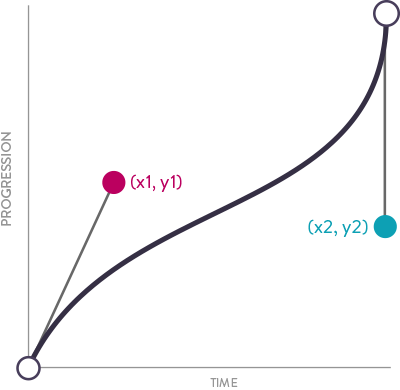
\includegraphics[keepaspectratio,width=\hsize,height=\halfh]
{images/cubicBezier.png}

\caption[Cubic-bezier Function]{
With coordinates for the location of the start and end weight we can define the desired function curve for progression through time by how much each half of the function should be deformed away from a linear function \citep{head2016designing}.
\imgcredit{The image is from the book
"Designing interface animation" by \citet{head2016designing}, used under CC BY 2.0 / It is accessible at {\em{}https://www.flickr.com/photos/rosenfeldmedia/albums/72157671107313626}.
}}
\label{fig:curve}
\end{figure}

While the animation properties just link the element to the desired changes, the actual CSS changes are defined in the @keyframes rule. In the rule we can set the keyframes, that are the finishing times, when a change should end. The keyframe times are simply described with percantage from 0\% as the start keframe and 100\% as the end keyframe. To this times we simply set, which styles should be used at the appointed time. The interpolation function set in with animation property will during proccessing interpolate the undefined percantages. For a better understanding see listing \ref{list:nonmotionAnime}.


\begin{lstlisting}[
language=CSS,
label=list:BibACMIEEE,
caption={[Example of non-motion animation in CSS]%
Simple example of non-motion animation with animation property and keyframes rule. A working example can be found between the attached code examples under nonmotionAnimationCSS.html.
}
]
div{
	animation: desiredName 4s linear 0s infinite alternate;
}

@keyframes desiredName {
	0%   {background-color:red;opacity: 1;transform: scale(1);}
	25%  {background-color:yellow;transform: scale(0.8);}
	50%  {background-color:blue;transform: scale(1);}
	75%  {background-color:green;transform: scale(1.5);}
	100% {background-color:red;opacity: 0.2;transform: scale(2);}
}
\end{lstlisting}
\label{list:nonmotionAnime}
% subsection CSS_animation_keyframe (end)

\subsection{Transition Property and Selector Pattern} % (fold)
\label{sub:CSS_transition}

The transition property can be used the same way as th animation property for defining the linking and interpolation details. There are even similarities int hte properties:

\begin{description}
\item [transition-property:] With this property we can link the the transition to a change in CSS, similar as with animation-name. However here we specify which of the CSS properties of the element should be interpolated during the change. It can be one or more properties seperated with a comma. We also have the default option none and convenient all, that sets all propertis to interpolate.
\item [transition-duration:] Same as animation-duration property.
\item [transition-timing-function:] Same as animation-timinig-function property.
\item [transition-delay:] Same as animation-delay property.
\end{description}

The unified property is also defined by the same order, with just less options:

\begin{description}
\item [transition:] property duration timing-function delay;
\end{description}

One can imagine the transition being a simplified version of the animation property, that can only have two keyframe, namely the start and end of the aniamtion or transtion. The start keyframe style is defined in the CSS style of the unchanged element, while the end frame is defined in a declaration where the specified transition property is changed. The easiest way to control such animations is with event seperators, such as :hover. This way we can define an animation to happen after hovering over the element. Since we can define just two keyframes and there ano repetitions, we are quite limited with the possible animations, which is also the reason for the animation property and keyframes rule to be used most of the time for animations. The limitations can be easily observed, when comparing the codes and results for \ref{list:nonmotionAnime} and \ref{list:nonmotionTransiton}.

\begin{lstlisting}[
language=CSS,
label=list:BibACMIEEE,
caption={[Example of non-motion transition in CSS]%
Simple example of non-motion animation with transition property and hover selector. A working example can be found between the attached code examples under nonmotionTransitionCSS.html.
}
]
div{
	background-color: red;
	opacity: 1;
	transition: all 4s;
}
div:hover{
	background-color:green;
	opacity: 0.2;
	transform: scale(2);
}
\end{lstlisting}
\label{list:nonmotionTransiton}

% subsection CSS_transition (end)

% section declarationCSS (end)

\subsection{Powerful Effect from Single Property} % (fold)
\label{sub:transformCSS}

While any CSS property can be defined for the animated change, there are some that can bring much more effect than others. Such would be the transform property, that can define translation, trotation and scalation in 2D and 3D space, plus also having options for skewing and puting into perspective the element. What is even more, is that all can be achieved at the same time. Just with combining it with the transform-origin property any kind of motion animation can be achieved.

% subsection transformCSS (end)


\section{CSS Examples} % (fold)
\label{sec:CSS_Examples}

While the previous sections tell us why animation can be useful, why CSS should be used and how to declare animation in CSS, we have yet to see CSS examples that show the difficulty to implement animation that brings benifits to the UI.
% section CSS_Examples (end)

\subsection{Navigation Animation} % (fold)
\label{sub:navigationCSS}

As stated in section \ref{sec:anime_why}, animation can help with navigation through the page. In the code examples we show two typical cases of such usage, namely the famous hamburger icon and menu position animation.

\subsubsection{Hamburger Icon} % (fold)
\label{subsub:hamburger}

The name comes from the icon being a set of three horizontal parallel lines sticking close together, the same way as the hamburger patty and meet sticks together. The icon is a metaphor for the menu to be tightly packed together, when we hide it "within" the icon. From the metaphor we also see the usefulness of such a concept, being the saving of space with hiding the menu and by showing the menu showing also the navigation path we are taking.

Implementations use various kinds of animations to make the use of the icon subtile and easy to use. Usually it is doen by rotating the lines in the icon into an X for showing the way of hiding or closing the menu and a sliding animation of the menu apearring from the border to show the navigation flow. An example of implementaations can be also observed in the code examples hamburgerVariationCSS.html and hamburgerMenuCSS.html, which are based on the code snippets provided by \citet{hamburgerMenu,hamburgerVar}.

By the information provided by \citet{vtldesign}, it is believed that the origins of the concept go back to 1981 and the famous company Xerox. However the explosion of usage came into being in the last decade, when designers were face with the problem of small screens on mobile devices.

\begin{lstlisting}[
language=CSS,
label=list:BibACMIEEE,
caption={[Example of Hamburger Icon in CSS]%
Extracted key HTML structure and CSS code for rotating the icon into an X. For details check code example hamburgerMenuCSS.html.
}
]
HTML structure:
<!-- ICON -->
<div id="menu-button" role="button">
  <div class="hamburger"><div class="inner"></div></div>
</div>
<!-- HIDDEN MENU -->
<nav><ul>
    <li><a href="">Home Page</a></li>
    <li><a href="">Other stuff</a></li>
</ul></nav>
Key CSS:
  /*Creates the hamburger lines*/
  .hamburger::before, .hamburger::after, .hamburger .inner {
    transition: all 750ms ease-in-out; ...
  }
  /*Upper and bottom lines rotate into an X*/
  .paperNav-container:hover .hamburger::before {
    transform: translate3d(-4px, 1px, 0) rotateZ(-45deg);  
  }
  .paperNav-container:hover .hamburger::after {
    transform: translate3d(-4px, -1px, 0) rotateZ(45deg);  
  }
  /*Middle line rotates into a point*/
  .paperNav-container:hover .hamburger .inner {
    transform: rotateY(-90deg); 
  }\end{lstlisting}
\label{list:hamburger}

\begin{figure}[h]
\centering

\includegraphics[keepaspectratio,scale=0.5]{images/hamburgerVar.png}

\includegraphics[keepaspectratio,scale=0.5]{images/hamburgerMenu.png}

\caption[Hamburger Examples]{
One the left we have a screenshot of code example hamburgerVariationCSS.html, which shows some of the different ways how hamburger icons are animated. On the right side we have hamburgerMenuCSS.html, that demonstrates the showing and hiding of the menu by hovering over the hamburger icon.
\imgcredit{Screenshot taken by the authors of this survey. The code behind the pages is by using the \citet{hamburgerMenu,hamburgerVar} online snippets as a base.}
}
\label{fig:hamburger}
\end{figure}



\subsubsection{Current menu position indicator} % (fold)
\label{subsub:menu}

A common problem with big menus is to keep track, where we currently are. The usual solutions are making a CSS change on the currently hovered or selected element. This can barely be said to be an animation, since the transition is instant. But such solutions can be even further improved with small animations, that are just extended previous solutions with the transiton having a duration. With adding duration to the animation, the user does not need to find where the change happened but just by observing it becomes a natural knowledge to the user, which also reduces the memory load and adds continuity to the navigation process. Typical solutions are combinations of opacity changes and translations of lines or even the menu words themselves. Such solutions can be observed in the code example in navigation.html, which is based on the code snippets by \citet{menuIndex}.

\begin{lstlisting}[
language=CSS,
label=list:BibACMIEEE,
caption={[Example of Menu Animation in CSS]%
Extracted key HTML structure and CSS code for presenting a few animations for menu position. For details check code example navigation.html.
}
]
HTML structure:
<div class="container [color] [effectClass]">
	<a alt="HOME">HOME</a>
	<a alt="ABOUT">ABOUT</a>
	<a alt="CONTACT">CONTACT</a>
</div>
Key CSS:
  /* Line that transits slowly under the text*/
  div.[class] a:before, div.borderYtoX a:after
  {
    height: 100%; /*vertical*/
    width: 2px;   /*  line  */
    transition: all 0.3s; ...
  }
  div.topBotomBordersOut a:after
  {
    bottom: 0px;
    transform: translateY(-10px);
  }

  /*Text jumps out*/
  div.highlightTextOut a:before,
  div.highlightTextIn a:before
  {
      content: attr(alt);
      transition: all 0.3s;
      transform: scale(0.8);
      opacity: 0; ...
  } 
  div.highlightTextOut a:hover:before,
  div.highlightTextIn a:hover:before
  {
      transform: scale(1);
      opacity: 1;
  }

\end{lstlisting}
\label{list:menu}

% subsection navigationCSS (end)

\subsection{Loading Animation} % (fold)
\label{sub:loadingCSS}

Another important use of animation is user feedback, see \ref{sec:anime_why}. The most common case being loading animations, that give the user a confirmation that the process is running, to not worry him of possible invisible crashes. The variety of animations is big but most could be specified as a continues rotation or a continues movement, usually in the horizontal direction. It is important to note, that all provided examples are pure HTML and CSS, without any JavaScript or SVGs. This also shows how powerful CSS can be.

\subsubsection{Rotating Icon} % (fold)
\label{subsub:rotation_loader}
A quick look at listing \ref{list:rotatingLoad} shows that the needed structure is just a div that has either a curve border created or it has a background color added. The circle animation is done with rotation in 2D space, while the square animation is done with rotation in 3D space. Working code examples are present in circleRotate2DCSS.html and squareRotated3DCSS.html, which are built from snippets done by \citet{cirleLoader,otherLoaders}.

\begin{lstlisting}[
language=CSS,
label=list:BibACMIEEE,
caption={[Example of Rotating Loading Animation in CSS]%
The actual needed code for both rotation loading animations. Working examples can be seen in circleRotate2DCSS.html and squareRotated3DCSS.html.
}
]
HTML structure:
  <div class="loaderClass"></div>
Key CSS:
.circleLoader {
	border: 16px solid #f3f3f3; /* Light grey */
	border-top: 16px solid #3498db; /* Blue */
	border-radius: 50%; /*the border is turned into the circle*/
	width: 120px;
	height: 120px;
	animation: spin 2s linear infinite;
}
@keyframes spin {
	0% { transform: rotate(0deg); }
	100% { transform: rotate(360deg); }
}

.squareloader {
  width: 60px;
  height: 60px;
  margin: 60px;
  animation: rotate 1.4s infinite ease-in-out;
}
@keyframes rotate {
  0% { transform: perspective(120px) rotateX(0deg) rotateY(0deg);}
  50% { transform: perspective(120px) rotateX(-180deg) rotateY(0deg);
  }
  100% { transform: perspective(120px) rotateX(-180deg) rotateY(-180deg);}
}
\end{lstlisting}
\label{list:rotatingLoad}

\begin{figure}[h]
\centering

\includegraphics[keepaspectratio,width=\hsize,height=\halfh]
{images/rotatingLoad.png}

\caption[Rotational Loading Animation Examples]{
A screenshot of rotating loaders, with the left one being a circle rotated in 2D and the right one a square rotated in 3D. The example code is located in circleRotate2DCSS.html and squareRotated3DCSS.html.
\imgcredit{Screenshot taken by the authors of this survey. The code behind the pages is by using the \citet{cirleLoader,otherLoaders} online snippets as a base.}
}
\label{fig:rotationLoad}
\end{figure}

\subsubsection{Horizontal movement} % (fold)
\label{subsub:menu}
The most common continues movement loader are horizontal. Therefore we provided 3 different types of movement in horizontal direction, namely moving dots, a progressbar and pulz-like wave motion. The working examples can be found in  
movingDotsCSS.html, progressbarCSS.html and pulzLoadCSS.html, which wer built using the \citet{otherLoaders} online snippets as a base.

\begin{lstlisting}[
language=CSS,
label=list:BibACMIEEE,
caption={[Example of Continues Movement Loading Animation in CSS]%
Extracted key HTML structure and CSS code for dots, progressbar and pulz loader. For details check code example movingDotsCSS.html, progressbarCSS.html and pulzLoaderCSS.html.
}
]
HTML structure:
<div class="loaderClass"><div></div><div></div><div></div><div></div></div>
Key CSS:
.dotsLoader div {
	background-color: black;
	border-radius: 50%;
	animation: dots-move 4s infinite cubic-bezier(.2,.64,.81,.23); ...
}
.dotsLoader div:nth-child(2) {
	animation-delay: 150ms; /*Change delay per child*/
}
@keyframes dots-move {
	0% {left: 0%;}
	75% {left:100%;}
	100% {left:100%;}
}

.progressbarloader:before{
	display: block;
	position: absolute;
	left: -200px;
	width: 200px;
	height: 4px;
	background-color: #2980b9;
	animation: bar-loading 2s linear infinite;
}
@keyframes bar-loading {
  from {left: -200px; width: 30%;}
  50% {width: 30%;}
  80% { left: 50%;}
  95% {left: 120%;}
  to {left: 100%;}
}

.pulzLoader div {
	animation: pulz-loading 1s ease-in-out infinite; ...
}
.pulzLoader div:nth-child(1) {  
	background-color: #3498db;  /*Change color per child*/
	animation-delay: 0;     /*Change delay per child*/
}
@keyframes pulz-loading {
	0% { transform: scale(1);}
	20% { transform: scale(1, 2.2);}
	40% { transform: scale(1);}
}
\end{lstlisting}
\label{list:horizontalLoad}

\begin{figure}[h]
\centering
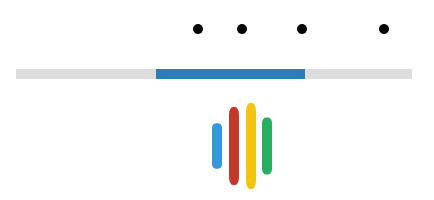
\includegraphics[keepaspectratio,width=\hsize,height=\halfh]
{images/horizontalLoad.png}

\caption[Continues Horizontal Movement Loading Examples]{
A screenshot of continues movement loaders in horizontal direction. On top we have animated dots that slow down in the middle of the animation. Second loader is the common progresbar, that is done by changing the left and width property. At the bottom we have an example of a pulz loader, that moves in wave form horizontaly and scales the bar when the "wave" comes. The example code is located in movingDotsCSS.html, progressbarCSS.html and pulzLoadCSS.html.
\imgcredit{Screenshot taken by the authors of this survey. The code behind the pages is by using the \citet{otherLoaders} online snippets as a base.}
}
\label{fig:rotationLoad}
\end{figure}

% section loadingCSS (end)